\documentclass[12pt]{report}
\usepackage{scribe,graphicx,graphics}
\usepackage{float}
\usepackage{siunitx}
\usepackage{braket}
\course{CSE 389D} 	
\coursetitle{Mathematical Modeling}	
\semester{Spring 2025}
\lecturer{} % Due Date: {\bf Mon, Oct 3 2016}}
\lecturetitle{Problem Set}
\lecturenumber{2}   
\lecturedate{}    
\usepackage{enumerate}
\newcommand{\remind}[1]{\textcolor{red}{\textbf{#1}}} %To remind me of unfinished work to fix later
\newcommand{\hide}[1]{} %To hide large blocks of code without using % symbols

\newcommand{\ep}{\varepsilon}
\newcommand{\vp}{\varphi}
\newcommand{\lam}{\lambda}
\newcommand{\Lam}{\Lambda}
%\newcommand{\abs}[1]{\ensuremath{\left\lvert#1\right\rvert}} % This clashes with the physics package
%\newcommand{\norm}[1]{\ensuremath{\left\lVert#1\right\rVert}} % This clashes with the physics package
\newcommand{\floor}[1]{\ensuremath{\left\lfloor#1\right\rfloor}}
\newcommand{\ceil}[1]{\ensuremath{\left\lceil#1\right\rceil}}
\newcommand{\A}{\mathbb{A}}
\newcommand{\B}{\mathbb{B}}
\newcommand{\C}{\mathbb{C}}
\newcommand{\D}{\mathbb{D}}
\newcommand{\E}{\mathbb{E}}
\newcommand{\F}{\mathbb{F}}
\newcommand{\K}{\mathbb{K}}
\newcommand{\N}{\mathbb{N}}
\newcommand{\Q}{\mathbb{Q}}
\newcommand{\R}{\mathbb{R}}
\newcommand{\T}{\mathbb{T}}
\newcommand{\X}{\mathbb{X}}
\newcommand{\Y}{\mathbb{Y}}
\newcommand{\Z}{\mathbb{Z}}
\newcommand{\As}{\mathcal{A}}
\newcommand{\Bs}{\mathcal{B}}
\newcommand{\Cs}{\mathcal{C}}
\newcommand{\Ds}{\mathcal{D}}
\newcommand{\Es}{\mathcal{E}}
\newcommand{\Fs}{\mathcal{F}}
\newcommand{\Gs}{\mathcal{G}}
\newcommand{\Hs}{\mathcal{H}}
\newcommand{\Is}{\mathcal{I}}
\newcommand{\Js}{\mathcal{J}}
\newcommand{\Ks}{\mathcal{K}}
\newcommand{\Ls}{\mathcal{L}}
\newcommand{\Ms}{\mathcal{M}}
\newcommand{\Ns}{\mathcal{N}}
\newcommand{\Os}{\mathcal{O}}
\newcommand{\Ps}{\mathcal{P}}
\newcommand{\Qs}{\mathcal{Q}}
\newcommand{\Rs}{\mathcal{R}}
\newcommand{\Ss}{\mathcal{S}}
\newcommand{\Ts}{\mathcal{T}}
\newcommand{\Us}{\mathcal{U}}
\newcommand{\Vs}{\mathcal{V}}
\newcommand{\Ws}{\mathcal{W}}
\newcommand{\Xs}{\mathcal{X}}
\newcommand{\Ys}{\mathcal{Y}}
\newcommand{\Zs}{\mathcal{Z}}
\newcommand{\ab}{\textbf{a}}
\newcommand{\bb}{\textbf{b}}
\newcommand{\cb}{\textbf{c}}
\newcommand{\db}{\textbf{d}}
\newcommand{\ub}{\textbf{u}}
\newcommand{\sbb}{\textbf{s}}
%\renewcommand{\vb}{\textbf{v}} % This clashes with the physics package (the physics package already defines the \vb command)
\newcommand{\wb}{\textbf{w}}
\newcommand{\xb}{\textbf{x}}
\newcommand{\yb}{\textbf{y}}
\newcommand{\zb}{\textbf{z}}
\newcommand{\vbb}{\textbf{v}}
\newcommand{\Ab}{\textbf{A}}
\newcommand{\Bb}{\textbf{B}}
\newcommand{\Cb}{\textbf{C}}
\newcommand{\Db}{\textbf{D}}
\newcommand{\eb}{\textbf{e}}
\newcommand{\ex}{\textbf{e}_x}
\newcommand{\ey}{\textbf{e}_y}
\newcommand{\ez}{\textbf{e}_z}
\newcommand{\zerob}{\mathbf{0}}
\newcommand{\abar}{\overline{a}}
\newcommand{\bbar}{\overline{b}}
\newcommand{\cbar}{\overline{c}}
\newcommand{\dbar}{\overline{d}}
\newcommand{\ubar}{\overline{u}}
\newcommand{\vbar}{\overline{v}}
\newcommand{\wbar}{\overline{w}}
\newcommand{\xbar}{\overline{x}}
\newcommand{\ybar}{\overline{y}}
\newcommand{\zbar}{\overline{z}}
\newcommand{\Abar}{\overline{A}}
\newcommand{\Bbar}{\overline{B}}
\newcommand{\Cbar}{\overline{C}}
\newcommand{\Dbar}{\overline{D}}
\newcommand{\Ubar}{\overline{U}}
\newcommand{\Vbar}{\overline{V}}
\newcommand{\Wbar}{\overline{W}}
\newcommand{\Xbar}{\overline{X}}
\newcommand{\Ybar}{\overline{Y}}
\newcommand{\Zbar}{\overline{Z}}
\newcommand{\Aint}{A^\circ}
\newcommand{\Bint}{B^\circ}
\newcommand{\limk}{\lim_{k\to\infty}}
\newcommand{\limm}{\lim_{m\to\infty}}
\newcommand{\limn}{\lim_{n\to\infty}}
\newcommand{\limx}[1][a]{\lim_{x\to#1}}
\newcommand{\liminfm}{\liminf_{m\to\infty}}
\newcommand{\limsupm}{\limsup_{m\to\infty}}
\newcommand{\liminfn}{\liminf_{n\to\infty}}
\newcommand{\limsupn}{\limsup_{n\to\infty}}
\newcommand{\sumkn}{\sum_{k=1}^n}
\newcommand{\sumk}[1][1]{\sum_{k=#1}^\infty}
\newcommand{\summ}[1][1]{\sum_{m=#1}^\infty}
\newcommand{\sumn}[1][1]{\sum_{n=#1}^\infty}
\newcommand{\emp}{\varnothing}
\newcommand{\exc}{\backslash}
\newcommand{\sub}{\subseteq}
\newcommand{\sups}{\supseteq}
\newcommand{\capp}{\bigcap}
\newcommand{\cupp}{\bigcup}
\newcommand{\kupp}{\bigsqcup}
\newcommand{\cappkn}{\bigcap_{k=1}^n}
\newcommand{\cuppkn}{\bigcup_{k=1}^n}
\newcommand{\kuppkn}{\bigsqcup_{k=1}^n}
\newcommand{\cappk}[1][1]{\bigcap_{k=#1}^\infty}
\newcommand{\cuppk}[1][1]{\bigcup_{k=#1}^\infty}
\newcommand{\cappm}[1][1]{\bigcap_{m=#1}^\infty}
\newcommand{\cuppm}[1][1]{\bigcup_{m=#1}^\infty}
\newcommand{\cappn}[1][1]{\bigcap_{n=#1}^\infty}
\newcommand{\cuppn}[1][1]{\bigcup_{n=#1}^\infty}
\newcommand{\kuppk}[1][1]{\bigsqcup_{k=#1}^\infty}
\newcommand{\kuppm}[1][1]{\bigsqcup_{m=#1}^\infty}
\newcommand{\kuppn}[1][1]{\bigsqcup_{n=#1}^\infty}
\newcommand{\cappa}{\bigcap_{\alpha\in I}}
\newcommand{\cuppa}{\bigcup_{\alpha\in I}}
\newcommand{\kuppa}{\bigsqcup_{\alpha\in I}}
\newcommand{\Rx}{\overline{\mathbb{R}}}
\newcommand{\dx}{\,dx}
\newcommand{\dy}{\,dy}
\newcommand{\dt}{\,dt}
\newcommand{\dax}{\,d\alpha(x)}
\newcommand{\dbx}{\,d\beta(x)}
\DeclareMathOperator{\glb}{\text{glb}}
\DeclareMathOperator{\lub}{\text{lub}}
\newcommand{\xh}{\widehat{x}}
\newcommand{\yh}{\widehat{y}}
\newcommand{\zh}{\widehat{z}}
\newcommand{\<}{\langle}
\renewcommand{\>}{\rangle}
\renewcommand{\iff}{\Leftrightarrow}
\DeclareMathOperator{\im}{\text{im}}
\let\spn\relax\let\Re\relax\let\Im\relax
\DeclareMathOperator{\spn}{\text{span}}
\DeclareMathOperator{\sym}{\text{Sym}}
\DeclareMathOperator{\myskew}{\text{Skew}}
\DeclareMathOperator{\Re}{\text{Re}}
\DeclareMathOperator{\Im}{\text{Im}}
\DeclareMathOperator{\diag}{\text{diag}}
\endinput

\theoremheaderfont{\itshape}
\theorembodyfont{\upshape}
\newtheorem{case}{Case}

% Insert your name here!
\scribe{Student Name: Noah Reef}
\newcommand{\rb}{\bold{r}}

\begin{document}
\maketitle
\section*{Problem 2.1}
\subsection*{Part a}
\begin{figure}[H]
    \centering
    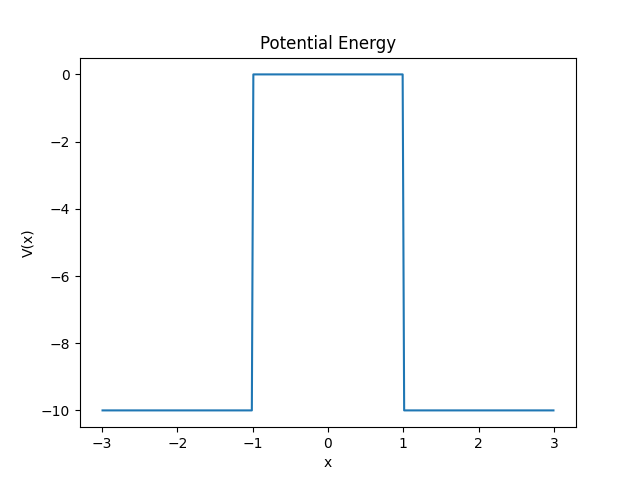
\includegraphics[scale=0.7]{Figure_1.png}
    \caption{Sketch of $V(x)$ for $a=1$,$b=3$, and $V_0 = 10$}
    \label{fig:enter-label}
\end{figure}
The time-independent Schrodinger's equation is given by
\begin{equation*}
    -\frac{\hbar^2}{2m} \frac{d^2\phi(x)}{dx^2} + V(x) \phi(x) = E\phi(x)
\end{equation*}

\subsection*{Part b}
If we consider the bounded state where $-V_0 < E < 0$, and $0 < x < a$, then we get that $V(x) = 0$ and
\begin{equation*}
    -\frac{\hbar^2}{2m} \phi''(x) = E \phi(x) \implies \phi''(x) = \frac{2m |E|}{\hbar^2} \phi(x)
\end{equation*}
solving the differential equation above gives the general solution,
\begin{equation*}
    \phi(x) = Ae^{\kappa x} + Be^{-\kappa x}
\end{equation*}
where
\begin{equation*}
    \kappa = \sqrt{\frac{2m |E|}{\hbar^2}}
\end{equation*}
however since it is symmetric we get that
\begin{equation*}
     \phi(x) = Ae^{\kappa x} + Ae^{-\kappa x} = 2A\cosh(\kappa x)
\end{equation*}
now if we consider the case where $a \leq x \leq b$, we have that $V(x) - V_0$ and get
\begin{equation*}
    -\frac{\hbar^2}{2m}\phi''(x) - V_0 \phi(x) = E\phi(x) \implies \phi''(x) = -\frac{2m(E + V_0)}{\hbar^2} \phi(x)
\end{equation*}
solving the above differential equation yields the following general solution
\begin{equation*}
    \phi(x) = C \cos(\xi (b-x)) + D \sin(\xi(b-x))
\end{equation*}
where 
\begin{equation*}
    \xi = \sqrt{\frac{2m(E + V_0)}{\hbar^2}}
\end{equation*}
then since $V(b) = \infty$ we require that $\phi(b) = 0$ and hence 
\begin{equation*}
    \phi(x) = D \sin(\xi (b-x))
\end{equation*}
now $x = a$ we have that
\begin{equation*}
    2A \cosh(\kappa a) = D \sin(\xi(b-a))
\end{equation*}
taking the derivatives 
\begin{equation*}
    2A\kappa \sinh(\kappa a) =  -D\xi\cos(\xi(b-a))
\end{equation*}
then dividing both equations yields
\begin{equation*}
    \frac{\kappa \sinh(\kappa a)}{\cosh(\kappa a)} = -\frac{\xi \cos(\xi(b-a))}{\sin(\xi(b-a))} \implies \kappa \tanh(\kappa a) = -\xi \cot(\xi (b-a)) = -\xi \frac{1 + \tan(\xi a)\tan(\xi b)}{\tan(\xi b) - \tan(\xi a)}
\end{equation*}
thus
\begin{equation*}
\kappa \tanh(\kappa a) + \xi \frac{1 + \tan(\xi a)\tan(\xi b)}{\tan(\xi b) - \tan(\xi a)} = 0
\end{equation*}
letting $v = \xi b$ and $a = \gamma b$ then we get that
\begin{equation*}
    \kappa \tanh(\kappa a) + (v/b) \frac{1 + \tan(\gamma v)\tan(v)}{\tan(v) - \tan(\gamma v)} = 0
\end{equation*}
note that if we define
\begin{equation*}
    S = \frac{b\sqrt{2mV_0}}{\hbar}
\end{equation*}
then we have that
\begin{align*}
    \kappa = \sqrt{\frac{2m|E|}{\hbar^2}} =\sqrt{\frac{2m(V_0 - (E + V_0)}{\hbar^2}} &= \sqrt{\frac{2mV_0}{\hbar^2} -\xi^2} \\
    &= \sqrt{\frac{2mV_0}{\hbar^2} -\frac{v^2}{b^2}} \\
    &= \frac{1}{b} \sqrt{S^2 - v^2}
\end{align*}
therefore we have that
\begin{equation*}
   \sqrt{S^2 - v^2} \tanh(\gamma \sqrt{S^2 - v^2}) - v \frac{1 + \tan(\gamma v)\tan(v)}{\tan(\gamma v) - \tan(v)} = 0
\end{equation*}
and hence our eigenvalues are given by
\begin{equation*}
    E + V_0 = \frac{\hbar^2 \xi^2}{2m} = \frac{\hbar^2 v^2}{2mb^2} \implies \frac{E}{V_0} = -1 + \frac{v^2}{S^2}
\end{equation*}
\subsection*{Part c}
Solving for $v$ from the equation below we get
\begin{align*}
    v_1 &= 9.87725 \\
    v_2 &= 6.84406 \\
    v_3 &= 3.46525 
\end{align*}
plugging these values into the equation
\begin{equation*}
    \frac{E}{V_0} = -1 + \frac{v^2}{S^2} 
\end{equation*}
yields
\begin{align*}
     \frac{E}{V_0} &= -1 + \frac{(9.87725)^2}{S^2} \approx -0.0244\\
      \frac{E}{V_0} &= -1 + \frac{(6.84406)^2}{S^2} \approx -0.5316\\
       \frac{E}{V_0} &= -1 + \frac{(3.46525)^2}{S^2} \approx -0.8799
\end{align*}
as the eigenvalues of the even bounded state problem.


\subsection*{Part d}
\subsection*{Part e}
To show the odd parity of the wave function we will get a similar result as in part b. However we notice that since the wave is odd we we get that in the case $|x| < a$ the wave function is given by
\begin{equation*}
  \phi(x) = Ae^{\kappa x} - Ae^{-\kappa x} = 2A\sinh(\kappa x)
\end{equation*}
and in the case $a < x < b$ we have that
\begin{equation*}
    \phi(x) = D \sin(\xi (b-x))
\end{equation*}
as before. Then we have that
\begin{align*}
  2A\sinh(\kappa a) &= D \sin(\xi(b-a)) \\
  2A\kappa \cosh(\kappa a) &= -D\xi\cos(\xi(b-a))
\end{align*}
then dividing the two equations yields
\begin{equation*}
    \frac{\kappa \cosh(\kappa a)}{\sinh(\kappa a)} = -\frac{\xi \cos(\xi(b-a))}{\sin(\xi(b-a))} \implies \kappa \coth(\kappa a) = -\xi \cot(\xi(b-a))
\end{equation*}
then by doing similar algebra and subsitutions as in part b we get that
\begin{equation*}
  \frac{\sqrt{S^2 - v^2}}{\tanh(\gamma \sqrt{S^2 - v^2})} - v \frac{\tan(\gamma v)\tan(v) + 1}{\tan(\gamma v) - \tan(v)} = 0
\end{equation*}
and hence the eigenvalues are given by 
\begin{equation*}
  \frac{E}{V_0} = -1 + \frac{v^2}{S^2}
\end{equation*}
as desired.

\subsection*{Part f}
Solving for $v$ from the equation below, using $S = 10$ and $\gamma = 0.2$ we get that
\begin{align*}
  v_1 &=   6.96192 \\
  v_2 &= 3.49913 \\
\end{align*}
plugging these values into the equation gives the following eigenvalues
\begin{align*}
  \frac{E}{V_0} &= -1 + \frac{(6.96192)^2}{S^2} \approx -0.5153\\
  \frac{E}{V_0} &= -1 + \frac{(3.49913)^2}{S^2} \approx -0.8775
\end{align*}

\subsection*{Part g}
The parity of the ground-state wavefunction is even.

\subsection*{Part h}

\subsection*{Part i}
Here we assume that the wavefunction is given in the form
\begin{equation*}
  \psi(x,t) = c_1(t) \psi_1(x) + c_2(t) \psi_2(x)
\end{equation*}
then we get that from the time-dependent Schrodinger's equation, that
\begin{align*}
  i\hbar \frac{d\psi}{dt} &= \hat{H}\psi \\
  i\hbar \frac{d}{dt} (c_1(t) \psi_1(x) + c_2(t)\psi_2(x)) = \hat{H}(c_1(t) \psi_1(x) + c_2(t)\psi_2(x)) \\
\end{align*}
which gives us
\begin{equation*}
  i\hbar \left(\frac{dc_1}{dt}\psi_1(x) + \frac{dc_2}{dt}\psi_2(x) \right) = \hat{H}(c_1(t) \psi_1(x) + c_2(t)\psi_2(x))
\end{equation*}
next we can multiply by $\psi_1^*(x)$ and $\psi_2^*(x)$ separately and integrate over all space to get the following
\begin{align*}
  i\hbar \dot{c}_1(t) &= \hat{H}c_1(t) = E_1c_1(t) \\
  i\hbar \dot{c}_2(t) &= \hat{H}c_2(t) = E_2c_2(t)
\end{align*}
solving the above differential equations gives us that
\begin{equation*}
  c_1(t) = c_1(0)e^{-iE_1t/\hbar} \quad c_2(t) = c_2(0)e^{-iE_2t/\hbar}
\end{equation*}
using the boundary conditions we get that
\begin{equation*}
  c_1(0) = \frac{1}{\sqrt{2}} \quad c_2(0) = \frac{1}{\sqrt{2}}
\end{equation*}
and thus the full solution is given by
\begin{equation*}
  \psi(x,t) = \frac{1}{\sqrt{2}}\left(e^{-iE_1t/\hbar}\psi_1(x) + e^{-iE_2t/\hbar}\psi_2(x)\right)
\end{equation*}

\subsection*{Part j}
If we suppose that the wavefunction is normalized at $t = 0$ then we have that
\begin{equation*}
  \int_{-\infty}^\infty |\psi(x,0)|^2 \, dx = 1
\end{equation*}
and thus for $t > 0$ we have that
\begin{align*}
  \int_{-\infty}^\infty \psi^*(x,t)\psi(x,t)\, dx = \frac{1}{2}\int_{-\infty}^\infty \psi_1^*(x)\psi_1(x) &+ \psi_2^*(x)\psi_2(x) + \psi_1^*(x)\psi_2(x)e^{i(E_1 - E_2)t/\hbar} \\ &+ \psi_2^*(x)\psi_1(x)e^{i(E_2 - E_1)t/\hbar} \, dx 
\end{align*}
and since $\psi_1$ and $\psi_2$ are orthogonal we get that
\begin{equation*}
  \int_{-\infty}^\infty \psi^*(x,t)\psi(x,t)\, dx = \frac{1}{2}\int_{-\infty}^\infty |\psi_1(x)|^2 + |\psi_2(x)|^2 \, dx = 1
\end{equation*}
and hence the wavefunction is normalized for all time.

\subsection*{Part k}
If we consider the probability density of $\psi$ we get that
\begin{align*}
  |\psi(x,t)|^2 &= \frac{1}{2}(|\psi_1(x)|^2 + |\psi_2(x)|^2 + \psi^*_1(x)\psi_2(x)e^{i(E_1 - E_2)t/\hbar} + \psi^*_2(x)\psi_1(x)e^{i(E_2 - E_1)t/\hbar}) \\
                &= \frac{1}{2}(|\psi_1(x)|^2 + |\psi_2(x)|^2 + 2\Re\left(\psi^*_1(x)\psi_2(x)e^{i(E_2 - E_1)t/\hbar}\right)
\end{align*}
Then we see that when $t = \pi\hbar/(E_2 - E_1)$ we have that
\begin{equation*}
  |\psi(x,t)|^2 = \frac{1}{2}|\psi_1(x) + \psi_2(x)|^2
\end{equation*}
and for $t = -\pi\hbar/(E_2 - E_1)$ we have that
\begin{equation*}
  |\psi(x,t)|^2 = \frac{1}{2}|\psi_1(x) - \psi_2(x)|^2
\end{equation*}
and hence has a period
\begin{equation*}
  T = \frac{2\pi\hbar}{E_2 - E_1}
\end{equation*}

\subsection*{Part l}


\section*{Problem 2.2}
\subsection*{Part a}
Recall that the expectation value of the electron distance from the nucleus in state $\psi_{nlm}$ is given by
\begin{equation*}
  r_{nlm} = \int r |\psi_{nlm}|^2 \, d\bold{r} = n^2 \left\{ 1 + \frac{1}{2} \left[1 - \frac{l(l+1)}{n^2}\right]\right\} a_0
\end{equation*}
where $a_0$ is the Bohr radius. For s-states we have that $l = 0$ and hence $m=0$ and thus $r_{n00} = \frac{3}{2}n^2 a_0$. So we have that the expectation value of the electron distance from the nucleus are
\begin{align*}
  r_{100} &= \frac{3}{2} a_0 \\
  r_{200} &= 6 a_0 \\
  r_{300} &= \frac{27}{2} a_0
\end{align*}
for the $1s-,2s-,3s-$states respectively.

\subsection*{Part b}
Recall that $a_0 = 0.0529177 \si{nm}$ and hence we get that the expectation values in part a are
\begin{align*}
  r_{100} &= 0.07937655 \si{nm} \\
  r_{200} &= 0.3175062 \si{nm} \\
  r_{300} &= 0.71438895\si{nm}
\end{align*}

\subsection*{Part c}
To show that the $1s$-state and $2s$-state are orthogonal we check to see if their inner product is $0$. First notice that
\begin{align*}
  \psi_{100} &= R_{10}(r)Y_{00}(\theta,\phi) \\
  \psi_{200} &= R_{20}(r)Y_{00}(\theta,\phi)
\end{align*}
then we have that
\begin{align*}
  \int_0^\infty \int_0^\pi \int_0^{2\pi} r^2 \sin(\theta) \psi_{100}^* \psi_{200} \, dr d\theta d\phi &= \int_0^\infty \int_0^\pi \int_0^{2\pi} R_{10}^* R_{20} r^2 |Y_{00}|^2 \sin(\theta) \, dr d\theta d\phi \\  
                                                                                                      &= \int_0^\infty R_{10}^* R_{20} \, dr\\
\end{align*}
and note that
\begin{align*}
  R_{10} &= 2a_0^{-3/2} e^{-r/a_0} \\ 
  R_{20} &= \frac{1}{\sqrt{2}} a_0^{-3/2} \left(1 - \frac{r}{2a_0}\right) e^{-r/2a_0}
\end{align*}
and hence our integral becomes
\begin{equation*}
  \int_0^\infty R_{10}^* R_{20} \, dr = \frac{2a_0^{-3}}{\sqrt{2}}\int_0^\infty r^2\left(1 - \frac{r}{2a_0} e^{\frac{-3r}{2a_0}}\right) \, dr  
\end{equation*}
using Mathematica to evaluate the integral, we get that
\begin{equation*}
  \int_0^\infty r^2\left(1 - \frac{r}{2a_0}\right) e^{\frac{-3r}{2a_0}} \, dr  = 0
\end{equation*}
and hence
\begin{equation*}
  \int_0^\infty \int_0^\pi \int_0^{2\pi} r^2 \sin(\theta) \psi_{100}^* \psi_{200} \, dr d\theta d\phi = 0
\end{equation*}
thus $\psi_{100}$ and $\psi_{200}$ are orthogonal.

\subsection*{Part d}
To show that the $2s$-state and the $2p$-states are orthogonal we aim to show that their inner product is zero. First recall that
\begin{align*}
  \psi_{200} &= R_{20}(r)Y_{00}(\theta,\phi) \\
  \psi_{21m} &= R_{21}(r)Y_{1m}(\theta,\phi)
\end{align*}
then we have that 
\begin{align*}
  \int_0^\infty \int_0^\pi \int_0^{2\pi} r^2 \sin(\theta) \psi_{21m}^* \psi_{200} \, dr d\theta d\phi &= \int_0^\infty \int_0^\pi \int_0^{2\pi} R_{20}^* R_{21} r^2 Y^*_{00}Y_{1m} \sin(\theta) \, dr d\theta d\phi \
\end{align*}
and since
\begin{equation*}
  \int_0^{\pi} \int_0^{2\pi} Y^*_{00}Y_{1m} \sin(\theta) \, d\theta d\phi = \delta_{01} \delta_{m0} = 0
\end{equation*}
and hence our above integral becomes
\begin{equation*}
  \delta_{01} \delta_{m0}\int_0^\infty R_{20}^* R_{21} r^2 \, dr = 0
\end{equation*}
thus $\psi_{200}$ and $\psi_{21m}$ are orthogonal for all $m$.

\section*{Problem 2.3}
\subsection*{Part a}
We consider 
\begin{equation*}
  \left[\frac{-\hbar^2}{2m} \nabla^2 - \frac{e^2}{4\pi \epsilon_0} + e \varepsilon x\right] \ket{\psi} = E \ket{\psi}
\end{equation*}
and assume that $\psi = c_1 \psi_{1s} + c_2 \psi_{2x}$. Then we have that
$\braket{\psi_{1s}|\psi} = c_1$ and $\braket{\psi_{2x}|\psi} = c_2$ since the $\psi_{1s}$ and $\psi_{2x}$ are orthonormal. Then we have that
\begin{align*}
\bra{\psi_{1s}}H\ket{\psi} = c_1\bra{\psi_{1s}}H\ket{\psi_{1s}} + c_2\bra{\psi_{1s}}H\ket{\psi_{2x}} = \bra{\psi_{1s}} E \ket{\psi} = c_1 E\\
\end{align*}
and
\begin{align*}
  \bra{\psi_{2x}}H\ket{\psi} = c_1\bra{\psi_{2x}}H\ket{\psi_{1s}} + c_2\bra{\psi_{2x}}H\ket{\psi_{2x}}   &= \bra{\psi_{2x}} E \ket{\psi} = c_2E\\
\end{align*}
where 
\begin{equation*}
  H =\frac{-\hbar^2}{2m} \nabla^2 - \frac{e^2}{4\pi \epsilon_0} + e \varepsilon x
\end{equation*}
Note that
\begin{equation*}
  \left(\bra{\psi_{1s}}H\ket{\psi_{2x}} \right)^* = \bra{\psi_{2x}}H\ket{\psi_{1s}}
\end{equation*}
and hence by letting
\begin{align*}
  h_{11} &= \bra{\psi_{1s}}H\ket{\psi_{1s}} \\
  h_{22} &= \bra{\psi_{2x}}H\ket{\psi_{2x}} \\
  h_{12} &= \bra{\psi_{1s}}H\ket{\psi_{2x}} = e\varepsilon \braket{\psi_{1s}|x|\psi_{2x}}
\end{align*}
we get that
\begin{equation*}
  \begin{pmatrix}
    h_{11} & h_{12} \\
    h_{12}^* & h_{22}
  \end{pmatrix}
  \begin{pmatrix}
    c_1 \\
    c_2
  \end{pmatrix}
  = E
  \begin{pmatrix}
    c_1 \\
    c_2
  \end{pmatrix}
\end{equation*}

\subsection*{Part b}
Recall that
\begin{equation*}
  \begin{cases}
    \psi_{1s} &= R_{10}(r)Y_{00}(\theta,\phi) \\
    \psi_{2p_x} &= \frac{R_{21}(r)}{\sqrt{2}} \left(Y_{1,-1}(\theta,\phi) - Y_{1,1}(\theta, \phi)\right)
  \end{cases}
\end{equation*}
Note that
\begin{align*}
  R_{10}(r) &= 2a_0^{-3/2} e^{-r/a_0} \\
  R_{21}(r) &= \frac{1}{\sqrt{6}}a_0^{-3/2}\left(\frac{r}{2a_0}\right)e^{-r/2a_0}\\
  Y_{1,-1} &= \sqrt{\frac{3}{8\pi}}e^{-i\phi}\sin(\theta) \\
  Y_{1,1} &= -\sqrt{\frac{3}{8\pi}}e^{i\phi}\sin(\theta) \\
  Y_{0,0} &= \sqrt{\frac{1}{4\pi}}
\end{align*}
and so we have that
\begin{equation*}
  \begin{cases}
    \psi_{1s} &= \frac{2}{\sqrt{4\pi}}a_0^{-3/2} e^{-r/a_0} \\ 
  \psi_{2px} &= \frac{1}{\sqrt{32\pi}} a^{-3/2}\left(\frac{r}{a_0}\right)e^{-r/2a_0}}\sin(\theta)\cos(\phi)
  \end{cases}
\end{equation*}
so then we have that
\begin{align*}
  \bra{\psi_{1s}}x\ket{\psi_{2p_x}} &= \int_0^\infty \int_0^\pi \int_0^{2\pi} r\sin(\theta)\cos(\phi) \psi_{1s}^* \psi_{2p_x} r^2\sin\theta \, dr d\theta d\phi \\
                                    &= \left(\frac{2}{\sqrt{4\pi}}\right)\left(\frac{1}{\sqrt{32\pi}}\right)a_0^{-4} \int_0^\infty r^4 e^{-3r/2a_0} \, dr \int_0^\pi \sin^3(\theta) \, d\theta \int_0^{2\pi} \cos^2(\phi) \, d\phi \\
                                    &= \frac{128 \sqrt{6}}{243} a_0
\end{align*}
and hence $e\varepsilon \braket{\psi_{1s}|x|\psi_{2p_x}} = \frac{128 \sqrt{6}}{243} e\varepsilon a_0$

\subsection*{Part c}
We compute the eigenvalues of the matrix above by
\begin{equation*}
  \det\left(\begin{bmatrix} 
    h_{11} -E & h_{12} \\
    h_{12}^* & h_{22} - E
\end{bmatrix}\right) = 0 \implies (h_{11} - E)(h_{22} - E) - |h_{12}|^2 = E^2 - E(h_{11} + h_{22}) + h_{11}h_{22} - |h_{12}|^2 = 0
\end{equation*}
solving the above equation gives us the eigenvalues of the matrix as
\begin{equation*}
  E = \frac{h_{11} + h_{22}}{2} \pm \sqrt{\left(\frac{h_{11} + h_{22}}{2}\right)^2} - (h_{11}h_{22} - |h_{12}|^2)
\end{equation*}
we take the $(-)$ term to get the lower energy eigenvalue. Then we get that
\begin{align*}
  c_1 h_11 + c_2 h_{12} &= E c_1 \\ 
  c_1 h^*_{12} + c_2 h_{22} &= E c_2
\end{align*}
Letting $c_1 = 1$ we get that
\begin{align*}
  c_2 &= \frac{E-h_{11}}{h_{12}} \\
\end{align*}
and hence we have 
\begin{equation*}
  \psi = \psi_{1s} + \frac{E - h_{11}}{h_{12}}\psi_{2p_x}
\end{equation*}
then normalizing the wavefunction gives us that
\begin{equation*}
  \psi = \frac{1}{\sqrt{1 + \frac{(E - h_{11})^2}{h_{12}^2}}}\left(\psi_{1s} + \frac{E - h_{11}}{h_{12}}\psi_{2p_x}\right)
\end{equation*}

\subsection*{Part d}

\subsection*{Part e}
Computing the dipole moment $\mu$ we get that
\begin{align*}
  \mu = -e\bra{\psi}x\ket{\psi} &= -e \left[\bra{\psi_{1s}}x\ket{\psi_{1s}} + M^2 \bra{\psi_{2p_x}}x\ket{\psi_{2p_x}} + M \bra{\psi_{1s}}x\ket{\psi_{2p_x}} + M \bra{\psi_{2p_x}}x \ket{\psi_{1s}}\right] \\
                                &= -2eM \bra{\psi_{1s}}x\ket{\psi_{2p_x}} \\
\end{align*}
where 
\begin{equation*}
  M = \frac{h_{12}}{h_{11} - h_{22}}
\end{equation*}
and get 
\begin{equation*}
  \mu = \frac{-2e^2\varepsilon}{h_{11} - h_{22}} \left(\frac{128 \sqrt{6}}{243} a_0\right)^2
\end{equation*}

\subsection*{Part f}
We have that
\begin{equation*}
  \alpha =\frac{2e^2}{h_{22} - h_{11}} \left(\frac{128\sqrt{6}}{243}\right)^2 
\end{equation*}
and 
\begin{equation*}
  \frac{ \alpha}{4\pi \epsilon_0} \approx \frac{4}{3}\frac{2e^2}{4\pi \epsilon_0E_{ha}} \left(\frac{128\sqrt{6}}{243}\right)^2 \left(a_0\right)^2 \approx a_0^3 \frac{8}{3}\left(\frac{128\sqrt{6}}{243}\right)^2 = 4.439 a_0^3 
\end{equation*}
which is close to experimental value of $4.61 a_0^3$.
\section*{Problem 2.4}
Let $\hat{P}$ be the parity operator, that is $\hat{P}f(r) = f(-r)$. Then if $f$ is an eigenfunction of $\hat{P}$ with eigenvalue $p$ then we have that
\begin{equation*}
  \hat{P}f(r) = f(-r) = \lambda f(r)
\end{equation*}
and 
\begin{equation*}
  \hat{P}^2 f(r) = f(-(-r)) = f(r) = \lambda^2 f(r) \implies \lambda^2 = 1
\end{equation*}
and hence $\lambda = \pm 1$. In the case $\lambda =1 $ we have that
\begin{equation*}
  f(r) = f(-r)
\end{equation*}
which implies that $f$ is an even function. Similarly for the case $\lambda = -1$ we have that
\begin{equation*}
  -f(r) = f(-r)
\end{equation*}
which implies that $f$ is an odd function. Thus our eigenvalues are $\pm 1$ and the eigenfunctions are even and odd functions respectively. 

\section*{Problem 2.5}
\subsection*{Part a}
If an operator $\hat{A}$ has eigenstates $\ket{a}$ with eigenvalues $\alpha$ then we have that 
\begin{equation*}
  \hat{A}\ket{a} = \alpha \ket{a}
\end{equation*}
additionally recall that the Taylor Expansion of $e^x$ is given by
\begin{equation*}
  e^x = \sum_{n=0}^\infty \frac{x^n}{n!}
\end{equation*}
and so 
\begin{equation*}
  e^{\hat{A}}\ket{a} = \sum_{n=0}^\infty \frac{\hat{A}^n}{n!}\ket{a} = \sum_{n=0}^\infty \frac{\alpha^n}{n!}\ket{a} = e^\alpha \ket{a}
\end{equation*}

\subsection*{Part b}
Recall that $z$ component of the angular momentum operator is given by $\hat{L}_z = \hat{x}\hat{p}_y - \hat{y}\hat{p}_x$. Additionally recall that a wavefunction 
is given by
\begin{equation*}
  \psi(r,\theta,\psi) = \sum_{lm}R_{lm}(r)Y_{lm}(\theta,\psi)
\end{equation*}
and hence we have that
\begin{equation*}
  \hat{L}_z\psi(r,\theta,\psi) = \sum_{lm}R_{lm}(r)\hat{L}_zY_{lm}(\theta,\psi)
\end{equation*}
and since $Y_{lm}(\theta,\psi)$ are eigenfunctions of $\hat{L}_z$ we have that
\begin{equation*}
  \hat{L}_zY_{lm}(\theta,\psi) = m\hbar Y_{lm}(\theta,\psi)
\end{equation*}
and hence
\begin{equation*}
  \hat{L}_z\psi(r,\theta,\psi) = \sum_{lm}R_{lm}(r)m\hbar Y_{lm}(\theta,\psi)
\end{equation*}
and thus
\begin{equation*}
  e^{i\hat{L}_z\phi_0/\hbar}\psi(r,\theta,\psi) = \sum_{lm}R_{lm}(r)e^{im\phi_0}Y_{lm}(\theta,\psi)
\end{equation*}
However note that
\begin{equation}
  e^{im\phi_0} Y_{lm}(\theta,\psi) = (-1)^{(m+|m|)/2}\sqrt{\frac{2l + 1}{4\pi}\frac{(l-m)!}{(l+m)!}}P_l^m(\cos(\theta))e^{im\phi + \phi_0} = Y_{lm}(\theta,\psi + \phi_0)
\end{equation}
and hence
\begin{equation*}
  e^{i\hat{L}_z\phi_0/\hbar}\psi(r,\theta,\psi) = \sum_{lm}R_{lm}(r)Y_{lm}(\theta,\psi + \phi_0) = \psi(r,\theta,\psi + \phi_0)
\end{equation*}
and hence the operator $e^{i\hat{L}_z\phi_0/\hbar}$ is the operator that rotates the wavefunction by an angle $\phi_0$ about the $z$-axis.
\end{document}
